\label{sec:noise_simulation}

View demo code of this section: \demonotebook{03}{chapt03} \ \demonotebookgithub{03}{chapt03}

\subsubsection{Quantum Channel}
Due to quantum decoherence and coupling with the environment, errors often occur in current quantum computers during the calculation process. They occur in stages such as state preparation, quantum gate operation, and measurement. This is often called quantum noise. Quantum noise can be characterized by quantum channels. In quantum information theory, quantum channels refer to completely positive trace-preserving (CPTP) maps in the operator space, which can also be regarded as a quantum operation. All quantum channels can be represented by Kraus operators

\begin{equation}
    \Psi(\rho) = \sum_i K_i \rho K_i^\dagger,
\end{equation}

where $\Psi$ is a quantum channel, $\rho$ is a density matrix, and $\{K_i\}$ are Kraus operators of $\Psi$. The Kraus operators satisfy the completeness condition

\begin{equation}
    \sum_i K_i^\dagger K_i = I.
\end{equation}

In density matrix simulator \code{"mqmatrix"}, we support the simulation of quantum channels based on the above mathematical form. In addition to the density matrix method, in the state vector simulator \code{"mqvector"} in \MindQuantum, we also support the Monte Carlo method to simulate quantum channels. The noise gate will affect the qubits with a certain probability. By sampling the circuit multiple times, we can get the noise-containing simulation results of quantum circuits. This process is much closer to how a real quantum computer works.

The following quantum channels are implemented in \MindQuantum.

\PauliChannel: Pauli channel can be seen as Pauli operators randomly apply to a quantum state $\rho$ with respect to a probability distribution.
\begin{equation}
    \Psi(\rho) = (1-p_x-p_y-p_z) \rho + p_x X \rho X + p_y Y \rho Y + p_z Z \rho Z.
\end{equation}
It becomes \BitFlipChannel\ if only $p_x$ is nonzero. Similarly, \PhaseFlipChannel\ has only one nonzero value $p_z$ and \BitPhaseFlipChannel\ is nonzero $p_y$. A special case is, all Pauli operators have same probabilities, which is called \DepolarizingChannel. Depolarizing channel is widely used in the description of quantum noise. Here is the formula in 1-qubit case:
\begin{equation}
    \Psi(\rho) =  (1-p) \rho + \frac{p}{4}(I\rho I+X\rho X+Y\rho Y+Z\rho Z).
\end{equation}
Depolarizing channel in \MindQuantum\ also supports multiple qubits case.
\begin{lstlisting}
from mindquantum.core.gates import DepolarizingChannel
from mindquantum.core.circuit import Circuit
circ = Circuit()
circ += DepolarizingChannel(0.02).on(0)
circ += DepolarizingChannel(0.01, 2).on([0, 1])
\end{lstlisting}

Damping Channel: Common damping channels include \AmplitudeDampingChannel\ and \PhaseDampingChannel. The amplitude damping channel can describe the dissipation of system energy, while the phase damping channel describes the loss of quantum information without exchanging energy with environment.
Amplitude damping channel applies noise as:
\begin{gather*}
    \epsilon(\rho) = E_0 \rho E_0^\dagger + E_1 \rho E_1^\dagger
    \\
    \text{where}\ {E_0}=\begin{bmatrix}1 & 0               \\
        0 & \sqrt{1-\gamma}\end{bmatrix},
    \ {E_1}=\begin{bmatrix}0 & \sqrt{\gamma} \\
        0 & 0\end{bmatrix}.
\end{gather*}
Phase damping channel applies noise as:
\begin{gather*}
    \epsilon(\rho) = E_0 \rho E_0^\dagger + E_1 \rho E_1^\dagger
    \\
    \text{where}\ {E_0}=\begin{bmatrix}1 & 0               \\
        0 & \sqrt{1-\gamma}\end{bmatrix},
    \ {E_1}=\begin{bmatrix}0 & 0             \\
        0 & \sqrt{\gamma}\end{bmatrix}.
\end{gather*}

\KrausChannel: The custom single-bit quantum channel in \MindQuantum. It can be constructed by passing in the Kraus operators.
\begin{lstlisting}
from mindquantum.core.gates import KrausChannel
from mindquantum.core.circuit import Circuit
from cmath import sqrt
gamma = 0.5
kmat0 = [[1, 0], [0, sqrt(1 - gamma)]]
kmat1 = [[0, sqrt(gamma)], [0, 0]]
amplitude_damping = KrausChannel('damping', [kmat0, kmat1])
circ = Circuit()
circ += amplitude_damping.on(0)
\end{lstlisting}

\subsubsection{Channel Adder}
A real quantum chip is comprised of multiple qubits. Due to inherent variabilities in the manufacturing process, each qubit exhibits distinct sources of error. Furthermore, the errors associated with the same qubit vary when different quantum gates are applied. To faithfully replicate the errors inherent in a quantum chip, a precise error model must be thoughtfully engineered. Within \MindQuantum, we have developed a suite of tools, called Channel Adder, which facilitates the rapid construction of noise models. Through the Channel Adder, we can conveniently introduce distinct quantum channels after various quantum gates, each tailored to specific qubits, and utilize noisy simulators to simulate these noise models.

The \ChannelAdder class consists of three main functions: \code{_accepter()}, \code{_excluder()}, and \code{_handler(BasicGate)}. Their functionalities are as follows:
\begin{itemize}
    \item \code{_accepter()}: Returns a list of functions called the accept rule set, where each accept rule function takes a quantum gate as input. When the function returns True, it indicates that we can add a channel after that quantum gate.
    \item \code{_excluder()}: Returns a list of functions called the reject rule set, where each reject rule function takes a quantum gate as input. When the function returns True, it indicates that we reject adding a channel after that quantum gate.
    \item \code{_handler(BasicGate)}: Takes a quantum gate as input and returns a quantum circuit representing a custom channel added after the input quantum gate.
\end{itemize}

Take \BitFlipAdder as an example. This adder will add a bit flip channel after every quantum gate.
\begin{lstlisting}
from mindquantum.core.circuit import Circuit, BitFlipAdder

circ = Circuit().h(0).rx('a', 1).z(1, 0)
noise_model = BitFlipAdder(0.3, with_ctrl=False)
noise_circ = noise_model(circ)
print(noise_model)
\end{lstlisting}
The output is:
\begin{lstlisting}
BitFlipAdder<flip_rate=0.3, with_ctrl=False>
\end{lstlisting}
After applying the noise model to a circuit, a bit flip channel will add to each quantum gate, see Fig.~\ref{fig:bit_flip_adder}.
\begin{figure}
    \centering
    \begin{subfigure}{0.2\textwidth}
        \centering
        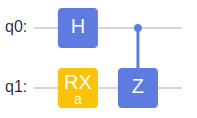
\includegraphics[width=\textwidth]{images/3_3_no_bit_fip.png}
        \caption{Circuit without noise.}
    \end{subfigure}
    \begin{subfigure}{0.4\textwidth}
        \centering
        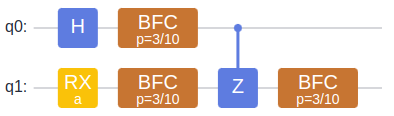
\includegraphics[width=0.9\textwidth]{images/3_3_bit_fip.png}
        \caption{Circuit after a \code{BitFlipAdder}.}
    \end{subfigure}
    \caption{An example of applying a BitFlipAdder to a quantum circuit.}
    \label{fig:bit_flip_adder}
\end{figure}

Here we will have a more complex example, so that we can see the power of Channel Adder. Assuming negligible noise in single-qubit gate operations on different qubits of the quantum chip, we consider that the two-qubit gates exhibit distinct depolarizing channel on different qubits. Additionally, the measurement of the circuit is subject to a bit-flip error with a flip probability of 0.01. We assume the depolarizing channels on different qubits to be:
\begin{lstlisting}
from mindquantum.core import *
dc0 = DepolarizingChannel(0.01)
dc1 = DepolarizingChannel(0.02)
dc2 = DepolarizingChannel(0.03)
\end{lstlisting}
Then we are going to build the whole noise model as:
\begin{lstlisting}
adder1 = MixerAdder([
    NoiseExcluder(),
    ReverseAdder(MeasureAccepter()),
    QubitNumberConstrain(2),
    NoiseChannelAdder(dc0, focus_on=0),
])
adder2 = MixerAdder([
    NoiseExcluder(),
    ReverseAdder(MeasureAccepter()),
    QubitNumberConstrain(2),
    NoiseChannelAdder(dc1, focus_on=1),
])
adder3 = MixerAdder([
    NoiseExcluder(),
    ReverseAdder(MeasureAccepter()),
    QubitNumberConstrain(2),
    NoiseChannelAdder(dc2, focus_on=2),
])
adder4 = MixerAdder([
    NoiseExcluder(),
    MeasureAccepter(),
    BitFlipAdder(0.01)
], add_after=False)

noise_model = SequentialAdder([
    adder1,
    adder2,
    adder3,
    adder4
])
print(noise_model)
\end{lstlisting}
The output is:
\begin{lstlisting}
SequentialAdder<
  MixerAdder<
    NoiseExcluder<>
    ReverseAdder<
      MeasureAccepter<>
    >
    QubitNumberConstrain<n_qubits=2, with_ctrl=True>
    NoiseChannelAdder<channel=DC(p=1/100), with_ctrl=True>
  >
  MixerAdder<
    NoiseExcluder<>
    ReverseAdder<
      MeasureAccepter<>
    >
    QubitNumberConstrain<n_qubits=2, with_ctrl=True>
    NoiseChannelAdder<channel=DC(p=1/50), with_ctrl=True>
  >
  MixerAdder<
    NoiseExcluder<>
    ReverseAdder<
      MeasureAccepter<>
    >
    QubitNumberConstrain<n_qubits=2, with_ctrl=True>
    NoiseChannelAdder<channel=DC(p=0.03), with_ctrl=True>
  >
  MixerAdder<
    NoiseExcluder<>
    MeasureAccepter<>
    BitFlipAdder<flip_rate=0.01, with_ctrl=True>
  >
>
\end{lstlisting}
A \MixerAdder is a set of adders, that all the \code{_accepter()} and\code{_excluder()} will be met. All the Channel Adder in \SequentialAdder will be executed one by one. From Fig.~\ref{fig:complex_adder}, we can see that this noise model satisfies our requirement.

% \begin{lstlisting}
% circ = Circuit().rx('a', 0).rx('b', 1).x(1, 0).rz('c', 1).x(1, 0).measure_all()
% \end{lstlisting}
\begin{figure}
    \centering
    \begin{subfigure}{0.32\textwidth}
        \centering
        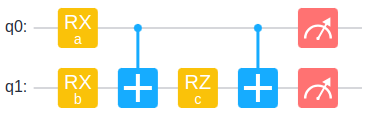
\includegraphics[width=\textwidth]{images/3_3_no_complex.png}
        \caption{Circuit without noise.}
    \end{subfigure}
    \begin{subfigure}{0.5\textwidth}
        \centering
        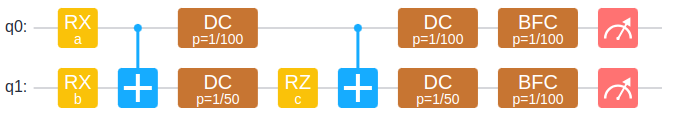
\includegraphics[width=\textwidth]{images/3_3_complex.png}
        \caption{Circuit after a complex Channel Adder.}
    \end{subfigure}
    \caption{An example of applying a complex Channel Adder to a quantum circuit.}
    \label{fig:complex_adder}
\end{figure}

After we build a noise model, we are easy to simulate a quantum circuit with this noise model in \MindQuantum.
\begin{lstlisting}
circ = Circuit().rx('a', 0).rx('b', 1).x(1, 0).rz('c', 1).x(1, 0).measure_all()
noise_sim = Simulator(NoiseBackend('mqvector', 2, noise_model))
noise_sim.sampling(circ, pr={'a': 1, 'b': 2, 'c':3}, shots=10000)
\end{lstlisting}
Here we construct a noise simulator using \code{"mqvector"}-based \NoiseBackend and the noise model that we built previously.
